\documentclass[12pt,a4paper]{article}
\usepackage[utf8]{inputenc}
\usepackage[left=2cm,right=2cm,top=2cm,bottom=2cm]{geometry}
\usepackage{amsfonts}
\usepackage{amsmath}
\usepackage{enumitem}
\usepackage{tikz}
\usepackage{pgfplots}

\newcommand{\set}[1]{\mathbb{#1}}
\newcommand{\pvec}[2]{\begin{pmatrix}#1\\#2\end{pmatrix}}
\newcommand{\module}[1]{\|#1\|}

\title{}
\author{-}
\date{2022 - 2023}

\pgfplotsset{compat=1.18}

\begin{document}

\maketitle
\section{Dades}
\begin{enumerate}[label=]
    \item - Qualitatives $\rightarrow$ No són numeros
    \item - Quantitatives $\rightarrow$ Són numeros
    \item \begin{enumerate}[label=-]
        \item Discretes $\rightarrow$ Numero enters
        \item Continues $\rightarrow$ Numeros decimals
    \end{enumerate}
\end{enumerate}

\subsection{Individu}
Element del qual en tinc informació
\subsection{Població}
Conjunt total d'individus d'un estudi
\subsection{Mostra}
Part representativa de tota la població que s'utilitza en cas de no poder accedir-hi.
\section{Parametres de posició}
$N$ el nomre total de dades
\begin{enumerate}[label=$\rightarrow$]
    \item Mediana: Valor que parteix les dades en 2 parts iguals\\[5pt]
        si $N$ Parell $Me=\frac{N}{2}$ i $\frac{N}{2}+1$, es igual a la mitjana aritmetica\\[5pt]
        si $N$ senar $Me=\frac{N}{2}+\frac{1}{2}$
    \item Quartils \begin{enumerate}[label=]
        \item Q1 - 25\% esquerra
        \item Q2 = Me
        \item Q3 - 25\% dreta
    \end{enumerate}
    \item Min/Max: El valor màxim i mínim
    \item Rang: $Es - Ei$
    \item Rang interquartil: $Q3 - Q1$
\end{enumerate}
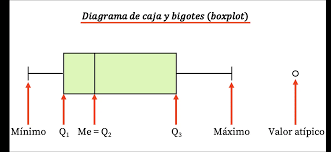
\includegraphics{Imatges/descarga.png}
\section{Centralització}
$x$: cada dada\\
$n$: freqüencia\\[10pt]
Mode: Dades més repetides Mo\\
Mitjana: $\overline{x}=\frac{1}{N}\sum x=\frac{1}{N}\sum n\cdot x$\\
Dispersió:
\begin{enumerate}[label=]
    \item Desviació mitjana DM\\[5pt]
        $DM = \frac{1}{N}\sum x-\overline{x}=\frac{1}{N}\sum\left(x-\overline{x}\right)\cdot n$
    \item Variança: $s^2$ per mostra, $\sigma^2$ per població\\[5pt]
        $s^2=\frac{1}{N-1}\sum\left(x-\overline{x}\right)^2=\frac{1}{N-1}\sum\left(x-\overline{x}\right)^2\cdot n$\\[5pt]
        $\sigma^2=\frac{1}{N}\sum\left(x-\overline{x}\right)^2=\frac{1}{N}\sum\left(x-\overline{x}\right)^2\cdot n$
\end{enumerate}
\subsection{Taula de freqüencia}
\begin{table}[!ht]
    \centering
    \begin{tabular}{|c|c|c|c|c|c|c|}
        $x$ & $n$ & $x\cdot n$ & $|x-\overline{x}|$ & $|x-\overline{x}|\cdot n$ & $\left(x -\overline{x}\right)^2$ &  $\left(x -\overline{x}\right)^2\cdot n$ \\ \hline
        4 & 2 & 8 & 1 & 2 & 1 & 2 \\ 
        5 & 3 & 15 & 0 & 0 & 0 & 0 \\ 
        6 & 2 & 12 & 1 & 2 & 1 & 2 \\ 
    \end{tabular}
\end{table}
\subsection{Desviació típica / estàndard}
$s =\sqrt{s^2}$\\[5pt]
$\sigma = \sqrt{\sigma^2}$
\subsection{Coaficient de variació}
$CV = \dfrac{s}{\overline{x}}$
\subsection{Covariança}
$S_{xy}$ o $\sigma_{xy}=\frac{1}{N}\sum\left(x-\overline{x}\right)\left(y-\overline{y}\right)$
\subsection{Coeficient Correlació lineal o de Perreson}
$\rho_{xy}=\dfrac{S_{xy}}{\sigma_{xy}}$\\[5pt]
$-1 \leq \rho \leq 1$
\section{Intervals}
En grups de dades molt grans utilitzem intervals semitancats, el petit inclos i el gran exclos.\\
Per $N$ dades, agrupo en $\sqrt{N}$ intervals (arrodonit).\\
L'amplitud d'un interval és $\dfrac{\text{rang}}{\sqrt{N}}$.\\
$x_i$: Marca de la mitjana aritmetica dels dos extrems de l'interval.\\
\subsection{Gràfics}
Diagrama de barres\\
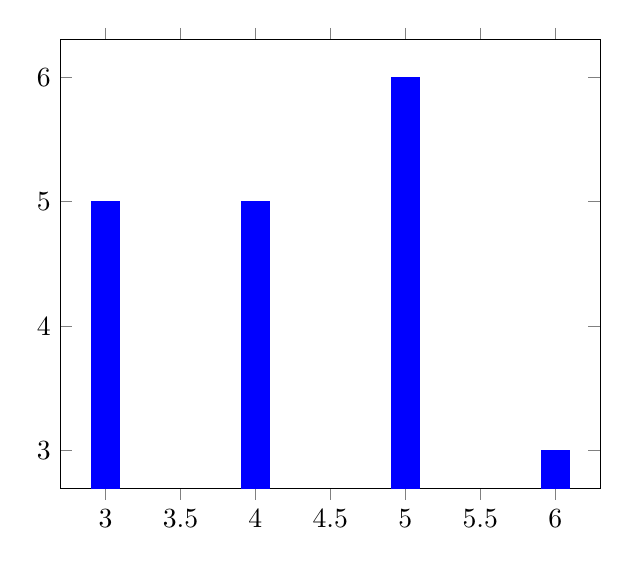
\begin{tikzpicture}
    \begin{axis}[ybar]
        \addplot[blue, fill=blue] plot coordinates
        {(3, 5) (4, 5) (5, 6) (6, 3)};
    \end{axis}
\end{tikzpicture}\\[5pt]
Istograma\\
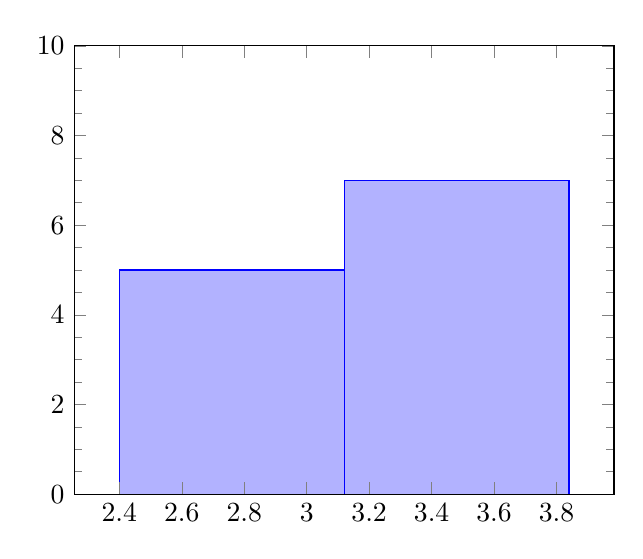
\begin{tikzpicture}
    \begin{axis}[
        ymin=0, ymax=10,
        minor y tick num = 3,
        area style,
    ]
    \addplot+[ybar interval, mark=no] plot coordinates
    {(2.40, 5) (3.12, 7) (3.84, 0)};
    \end{axis}
\end{tikzpicture}
\end{document}
